\documentclass[../TDE6_rsf.tex]{subfiles}%

\begin{document}
\section[s]"2"{Oscillateur à quartz}
\enonce{%
	\begin{minipage}{0.60\linewidth}
		Un quartz piézo-électrique se modélise par un condensateur (de capacité
		$C_0$) placé en parallèle avec un condensateur (de capacité $C$) en série
		avec une inductance $L$. On se place en régime sinusoïdal forcé de pulsation
		$\w$.
	\end{minipage}
	\hfill
	\begin{minipage}{0.35\linewidth}
		\begin{center}
			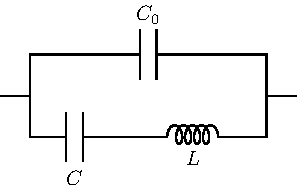
\includegraphics[width=\linewidth]{quartz_plain}
		\end{center}
	\end{minipage}
}

\QR{%
	Donner l'impédance équivalente $\Zu$ de l'oscillateur.
}{%
	On calcule l'association en série de $C$ et $L$ d'abord, puis on fait
	l'association en parallèle de ce dipôle avec $C_0$~:
	\begin{center}
		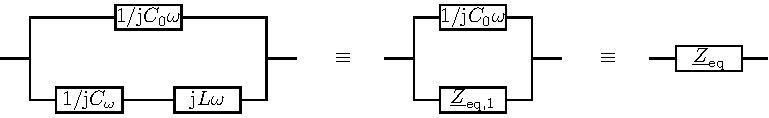
\includegraphics[width=\linewidth]{quartz_equiv}
	\end{center}
	\begin{isd}
		\begin{align*}
			\Zu\ind{eq, 1} & = \frac{1}{\jj C\w} + \jj L \w
			\\\beforetext{D'où}
			\Zu
			               & = \frac{1}{\Yu_{C_0} + \Yu\ind{eq, 1}}
			\\\Lra
			\Zu
			               & = \frac{1}{\jj C_0\w + \dfrac{1}{\frac{1}{\jj C\w} + \jj L\w}}
			\times
			\frac{\frac{1}{\jj C\w} + \jj L\w}{\frac{1}{\jj C\w} + \jj
				L\w}
			\\\Lra
			\Zu
			               & = \frac{\frac{1}{\jj C\w} + \jj L\w}{1 + \frac{C_0}{C} -
				LC_0\w^2}
			\times
			\frac{\jj C\w}{\jj C\w}
		\end{align*}
		\tcblower
		\begin{align*}
			\Lra
			\Zu
			    & = \frac{1 - LC\w^2}{\jj C\w + \jj C_0\w -\jj LCC_0\w^3}
			\\\Lra
			\Zu
			    & = -\jj \frac{1 - LC\w^2}{(C+C_0)\w - LCC_0\w^3}
			\\\Lra
			\Aboxed{%
			\Zu & =
				\jj \frac{LC\w^2 - 1}{\w\left((C+C_0) - LCC_0\w^2\right)}
			}%
		\end{align*}
	\end{isd}
}

\QR{%
	Trouver la pulsation pour laquelle l'impédance de l'ensemble est
	nulle, puis celle pour laquelle elle est infinie.
}{%
	L'impédance est nulle si le numérateur est nul, c'est-à-dire
	\[\boxed{\Zu = 0 \Lra \w = \w_0 = \sqrt{\frac{1}{LC}}}\]
	À cette pulsation, assimilable à la pulsation propre d'un circuit RLC
	série, le dipôle est donc équivalent à un fil. On retrouvera ce
	résultat en étudiant la résonance dans le chapitre suivant. \bigbreak
	L'impédance est infinie si le dénominateur est nul, c'est-à-dire
	\[\boxed{\abs{\Zu} \ra \infty \Lra \w = \w_0' =
			\sqrt{\frac{C+C_0}{LCC_0}}}\]
	Cette pulsation serait la pulsation propre d'une bobine $L$ et d'un
	condensateur de capacité $C\ind{eq} = \frac{CC_0}{C+C_0}$, autrement dit
	l'association en série d'un condensateur $C$ et d'un autre condensateur
	$C_0$ (les inverses des capacités s'ajoutent en série). \smallbreak
	À cette pulsation (dite «~de résonance~», cf.\ chapitre suivant), la
	bobine et les condensateurs se chargent et déchargent alternativement,
	l'énergie arrivant dans le dipôle est piégée et n'est pas transmise au
	reste du circuit, comme le fait un interrupteur ouvert.
}

\QR{%
	Tracer l'allure de $\abs{\Zu(\w)}$.
}{%
	\begin{minipage}[t]{0.55\linewidth}
		On regarde les cas limites à très haute et très basse fréquence~:
		\begin{gather*}
			\abs{\Zu} \xrightarrow[\w\ra\infty]{} 0
			\qet
			\abs{\Zu} \xrightarrow[\w\ra0^+]{} \infty
		\end{gather*}
		En effet, à $\w \ra 0$, les condensateurs sont des interrupteurs
		ouverts donc l'impédance totale est celle d'un interrupteur ouvert. À
		l'inverse, à $\w \ra \infty$, les condensateurs sont des fils
		donc l'impédance totale est celle d'un fil~: 0.
	\end{minipage}
	\hfill
	\begin{minipage}[t]{0.45\linewidth}
		\vspace{0pt}
		\begin{center}
			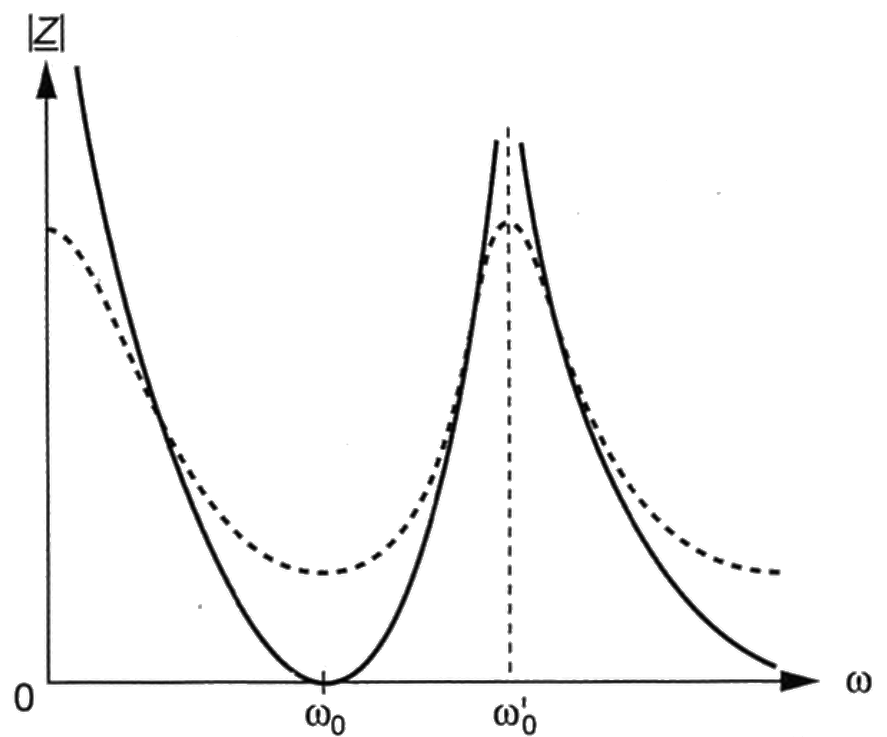
\includegraphics[width=\linewidth]{exo8_solve-clean}
		\end{center}
	\end{minipage}
}

\QR{%
	Comment la courbe précédente serait-elle modifiée si on prenant en
	compte les résistances de chacun des composants~?
}{%
	Les résistances évitent les infinités par dissipation, mais également
	les valeurs nulles~: on se retrouve avec la courbe en pointillés sur la
	figure précédente.
}
\end{document}
